%
% @file doc.tex
% @author David Kvaček (xkvace00@stud.fit.vutbr.cz)
% @brief Project simulation study from the IMS course.
% @date 2024-12-02
%

\documentclass[a4paper, 11pt]{article}
\usepackage[left=2cm, text={17cm, 25cm}, top=3cm]{geometry}
\usepackage[czech]{babel}
\usepackage[utf8]{inputenc}
\usepackage[IL2]{fontenc}
\usepackage{graphicx}
\usepackage{hyperref}

\begin{document}

\begin{titlepage}
    \begin{center}
        
\includegraphics[scale=0.125]{logo.png} \\
        \vspace{\stretch{0.382}}
        \LARGE{Simulační studie projektu z~předmětu IMS} \\
        \huge{\textbf{SHO Model v~průmyslové výrobě nebo zemědělství}} \\
        \LARGE{Tým xkvace00}
        \vspace{\stretch{0.618}}
    \end{center}

    \null \Large{\hfill David Kvaček} \\
    \Large{Brno, \today \hfill \href{mailto:xkvace00@stud.fit.vutbr.cz}{xkvace00@stud.fit.vutbr.cz}}
\end{titlepage}

\tableofcontents

\newpage

\section{Úvod}

V~rámci projektu předmětu Modelování a~simulace (IMS) na Fakultě informačních technologií Vysokého učení technického v~Brně je realizována simulační studie zaměřená na vytvoření modelu výrobního systému v~oblasti strojírenské výroby.
Hlavním cílem této práce je analyzovat a~optimalizovat výrobní proces konkrétního podniku Czech LANA s.r.o. se sídlem ve Ždírci nad Doubravou, přičemž pozornost je zaměřena na jeden konkrétní produkt.
Simulační model podrobně zkoumá provoz výrobní linky, pohyb materiálů a~interakci s~pracovníky.

Klíčovým úkolem této studie je odhalit nedostatky v~provozu zkoumaného podniku a~prostřednictvím simulací navrhnout úpravy a~změny, které by vedly k~efektivnějšímu a~lépe organizovanému výrobnímu procesu.
To zahrnuje například změny v~uspořádání výrobní linky, úpravě kapacit či dalších zásadních provozních parametrech.
Autor takto usiluje o~poskytnutí praktických a~využitelných poznatků, které přispějí ke zlepšení výrobního systému a~zvýšení jeho celkové efektivity.

\subsection{Autor práce a~zdroje informací}

Autorem této práce je David Kvaček, student třetího ročníku bakalářského studia na Fakultě informačních technologií Vysokého učení technického v~Brně.
Odbornou podporu a~klíčové informace poskytl pan Josef Pavel, vedoucí oddělení odpovědného za modelovaný úsek výrobního procesu.

Autor čerpá poznatky především z~osobní prohlídky pracoviště pod vedením odborné autority.
Nejasnosti, které vznikají během realizace studie, řeší prostřednictvím e-mailové komunikace s~panem Pavlem nebo se zástupci příslušného firemního úseku.

\subsection{Ověření validity modelu}

Významná část informací pochází přímo od odborného konzultanta spolupracující firmy.
Tento přístup zajišťuje požadovanou přesnost simulace a~souvisejících výstupů, které jsou předkládány panu Pavlovi k~posouzení.
Komunikace se zástupci modelovaného úseku výrobní linky zahrnuje diskusi nad výsledky a~statistikami, které se ukazují jako poměrně přesné.
Na základě těchto poznatků probíhá srovnání reálných dat z~prostředí firmy s~výstupy simulace, přičemž rozdíly mezi nimi jsou zanedbatelné.

\newpage

\section{Rozbor tématu a~použitých metod/technologií}

Téma projektu se zaměřuje na simulaci výrobní linky, tok materiálu a~součinnost s~pracovníky v~rámci vybrané části linky společnosti Czech LANA s.r.o.
Tato firma se specializuje na zpracování dřeva ve všech jeho podobách, je součástí mezinárodního koncernu a~řadí se mezi světové lídry ve svém oboru.

Simulační studie se soustředí na konkrétní fázi výrobního procesu.
Zpracované dřevěné hranoly, lišty a~podobné produkty putují po výrobní lince do zkoumaného úseku.
Tento úsek rozděluje přicházející výrobky (požadavky na zpracování) po určitém počtu tak, aby vzniklé části mohly být uspořádány na připravené rampy nebo palety.

Požadavky přicházejí s~určitou frekvencí, která je určena exponenciálním rozložením.
Jakmile je separováno určité množství výrobků, následuje proces umístění prokladových lišt na danou vrstvu výrobků.
Tuto fázi výrobního procesu zajišťují mechanické stroje s~určitou kapacitou, jež udávají maximální možné počty prokladových lišt, které mohou stroje pojmout.
Stroje však nepracují bezchybně a~v~intervalech definovaných exponenciálním rozložením dochází k~poruchám, které musí pracovník opravit (doba opravy závisí na závažnosti poruchy).

Hlavním úkolem zaměstnance je doplňování prokladových lišt do již zmíněných mechanických zařízení, přičemž tento proces je řízen exponenciálním rozložením, které závisí na velikosti, délce, tloušťce a~povrchu jednotlivých prokladových lišt.

\subsection{Popis použitých postupů}

K~popisu modelovaného problému je využita diskrétní simulace, která se pro tento účel ukazuje jako dostatečně robustní.
Simulace je implementována v~programovacím jazyce \texttt{C++} s~využitím specializované knihovny \texttt{SIMLIB}, navržené pro podobné aplikace.
Abstraktní model simulovaného procesu je vytvořen pomocí Petriho sítě.

\subsection{Popis původu použitých metod/technologií}

Implementace simulačního modelu využívá standardní funkce poskytované programovacím jazykem \texttt{C++}.
Současně je aplikována také doporučená knihovna \texttt{SIMLIB}.
Pro návrh abstraktního modelu jsou využity osvědčené metody modelování založené na Petriho sítích.

\newpage

\section{Koncepce modelu}

Jedním z~hlavních cílů simulační studie je zdokumentovat a~navrhnout efektivnější využití zdrojů potřebných pro zkoumanou část výrobního procesu.
Simulace se zaměřuje na část výrobní linky, kde pracují zaměstnanci, kteří se aktivně podílejí na provozu podniku.

Tato část výrobní linky je vybrána s~ohledem na její variabilitu oproti ostatním fázím výrobního procesu, které jsou většinou plně automatizované a~nevyžadují zásah pracovníků, což by umožnilo zkoumat především vzniklé poruchy.
Proto je zvolen kompromis, který však nemá zásadní dopad na výsledky studie.

Model je vytvořen s~využitím Petriho sítě (obrázek \ref{PetriNet}) obsahující dva generátory.
První generátor náhodně vytváří požadavky přicházející na výrobní linku, které reprezentují jednotlivé výrobky.
Tyto požadavky obsazují obslužnou linku a~odebírají prokladové lišty ze zásobníků o~daných kapacitách.
Po zpracování požadavku je obslužná linka uvolněna a~požadavek opouští systém.
Pokud se nějaký zásobník prokladových lišt vyprázdní, zaměstnanec zasahuje a~v~určitém časovém intervalu doplňuje zásobník na maximální kapacitu.

Současně pracuje druhý generátor, který simuluje poruchy obslužné linky.
V~okamžiku poruchy musí pracovník ihned zakročit, čímž se proces zpracování požadavků pozastaví, toto se projeví na následující položce.
Po odstranění poruchy výroba pokračuje opětovným zprovozněním obslužné linky, zatímco opravená porucha opouští systém.

\subsection{Abstraktní model --~Petriho síť}

\begin{figure}[ht]
    \centering
    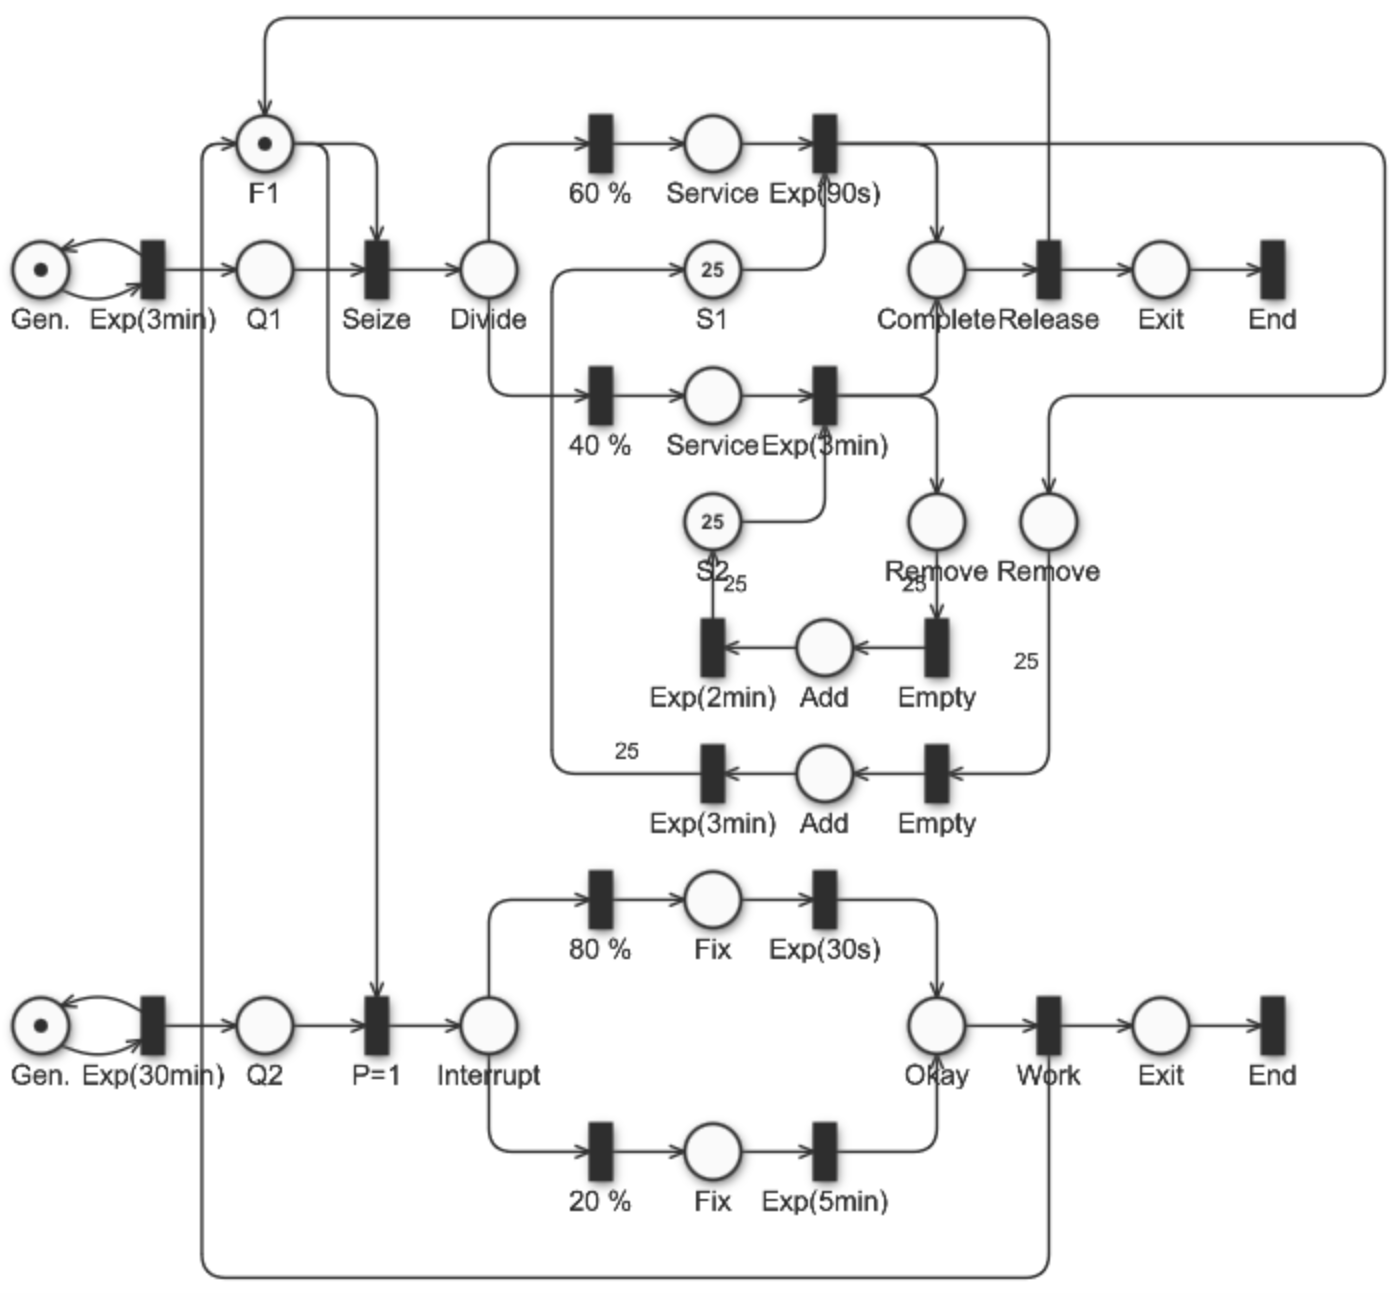
\includegraphics[width=0.86\textwidth]{petri-net.png}
    \caption{Abstraktní model v~Petriho síti.}
    \label{PetriNet}
\end{figure}

\newpage

\section{Architektura simulačního modelu}

Simulační program se skládá z~několika částí.
Nejprve jsou určeny klíčové konstanty, které vycházejí z~osobních zkušeností získaných konzultacemi se zástupci příslušného firemního oddělení.
Tyto hodnoty se následně přizpůsobují jednotlivým experimentům podle potřeb konkrétní analýzy.
Délka simulace je však pevně určena na osm hodin, což odpovídá jednomu pracovnímu dni (v~programu \texttt{28800} sekund), protože každá směna začíná ve stejné fázi jako ta předchozí.
Modelování více stejných pracovních dní proto nemá žádný praktický význam.
Následně se vytvářejí jednotlivé třídy, které slouží k~popisu událostí a~procesů aktivně ovlivňujících výsledky jednotlivých experimentů.

\subsection{Popis jednotlivých prvků architektury}

Klíčovou třídou je \texttt{Request}, která reprezentuje příchozí výrobní požadavky vstupující do systému.
Na začátku procesu se z~důvodu zaznamenávání statistik ukládá aktuální čas příchodu do systému do proměnné \texttt{Arrival}.
V~případě poruchy se proces přesouvá do fronty \texttt{Q1} a~je přerušen na neurčitou dobu, přičemž jeho opětovné spuštění zajišťuje proces řešení poruchy.
Dále proces zabírá obslužnou linku prostřednictvím metody \texttt{Seize}.

Příchozí požadavky mají dva možné typy -- běžné, nebo speciální.
Toto rozdělení je simulováno pomocí vestavěné funkce \texttt{Random}.
Pokud se stane, že je sklad \texttt{S1} pro běžné požadavky, nebo sklad \texttt{S2} pro speciální požadavky prázdný, proces čeká po určitou dobu, než odpovědný pracovník sklad opět doplní na plnou kapacitu.
V~opačném případě požadavek odebere jednu položku ze skladu \texttt{S1}, nebo \texttt{S2} a~pokračuje v~čekání na dokončení zpracování.
Nakonec proces uvolňuje obslužnou linku prostřednictvím metody \texttt{Release} a~úspěšně opouští systém.

Další významnou třídou je \texttt{Failure}, která zajišťuje simulaci poruch vznikajících ve výrobním procesu.
Na začátku se opět zaznamenává čas příchodu poruchy pro účely statistického vyhodnocení.
V~okamžiku výskytu poruchy se globální proměnná \texttt{failure} nastaví na pravdivostní hodnotu \texttt{true}.
Poruchy v~modelu mohou být buď nezávažné, nebo závažné.
Každý typ poruchy je po určité době odstraněn, globální proměnná \texttt{failure} se nastaví zpět na pravdivostní hodnotu \texttt{false}, a~pokud fronta pozastavených požadavků obsahuje procesy, aktivuje se první z~nich.

Následně přicházejí třídy událostí, které vytvářejí výše zmíněné procesy s~exponenciálním rozložením.
Hlavní funkce \texttt{main} inicializuje experiment odpovídající jednomu pracovnímu dni, aktivuje generátory a~spouští samotnou simulaci.
Po dokončení simulace vypisuje statistiky na standardní výstup.
Vstupní hodnoty jednotlivých experimentů, tedy různé hodnoty klíčových konstant, je nutné upravit přímo ve zdrojovém kódu, protože je nelze nastavit prostřednictvím příkazové řádky.

\newpage

\section{Podstata simulačních experimentů a~jejich průběh}

Experimenty jsou navrženy k~určení optimálního počtu zdrojů nezbytných pro efektivní provoz výrobního procesu.
Cílem je zjistit maximální kapacitu výrobní linky, kterou dokážou zvládnout dva mechanické stroje na prokladové lišty spolu s~jedním pracovníkem obsluhujícím linku.

\subsection{Postup experimentování}

První experiment slouží k~ověření, zda simulace odpovídá skutečnosti.
Toho se dosahuje nastavením klíčových konstant podle informací získaných od odborného konzultanta.
V~dalších experimentech se pak postupně mění jednotlivé klíčové konstanty, přičemž získané údaje o~provedených změnách slouží jako podklad pro následující experimenty.

\subsection{První experiment}

Tento experiment potvrzuje validitu modelu, jelikož všechny důležité statistiky v~přiměřeném rozsahu odpovídají reálným hodnotám.
Vstupní hodnoty parametrů simulačního modelu, uvedené v~následujícím výčtu, mají za následek odpovídající statistiky v~tabulce \ref{FirstExperiment}.\\ \\
\texttt{S1\_MAX = 25} --~maximální kapacita skladu prokladových lišt~1 (25\,ks),\\
\texttt{S2\_MAX = 25} --~maximální kapacita skladu prokladových lišt~2 (25\,ks),\\
\texttt{RG\_MEAN = 180} --~střední hodnota exp. rozložení generátoru vstupních požadavků (3\,min.),\\
\texttt{FG\_MEAN = 1800} --~střední hodnota exp. rozložení generátoru poruch linky (30\,min.),\\
\texttt{R\_TYPE = 0.6} --~průměrný počet běžných požadavků podle rovnoměrného rozložení (60\,\%),\\
\texttt{F\_TYPE = 0.8} --~průměrný počet nezávažných poruch podle rovnoměrného rozložení (80\,\%),\\
\texttt{R1\_MEAN = 90} --~střední hodnota exp. rozložení doby obsluhy běžných požadavků (1,5\,min.),\\
\texttt{R2\_MEAN = 180} --~střední hodnota exp. rozložení doby obsluhy speciálních požadavků (3\,min.),\\
\texttt{R1\_ADD = 60} --~střední hodnota exp. rozložení doby doplnění skladu 1~pracovníkem (1\,min.),\\
\texttt{R2\_ADD = 120} --~střední hodnota exp. rozložení doby doplnění skladu 2~pracovníkem (2\,min.),\\
\texttt{F1\_MEAN = 30} --~střední hodnota exp. rozložení doby opravy nezávažné poruchy (0,5\,min.),\\
\texttt{F2\_MEAN = 300} --~střední hodnota exp. rozložení doby opravy závažné poruchy (5\,min.).

\begin{table}[ht!]
    \centering
    \begin{tabular}{|l|r|}
        \hline
        Celkový počet vstupních požadavků & \textbf{134,00\,ks} \\ \hline
        Průměrná vytíženost obslužné linky \texttt{F1} & \textbf{55,71\,\%} \\ \hline
        Maximální délka fronty \texttt{Q1} & \textbf{8,00\,ks} \\ \hline
        Průměrná délka fronty \texttt{Q1} & \textbf{0,79\,ks} \\ \hline
        Minimální čas ve frontě \texttt{Q1} & \textbf{4,02\,s} \\ \hline
        Maximální čas ve frontě \texttt{Q1} & \textbf{959,19\,s} \\ \hline
        Průměrný čas ve frontě \texttt{Q1} & \textbf{285,84\,s} \\ \hline
        Minimální doba obsluhy požadavku & \textbf{10,30\,s} \\ \hline
        Maximální doba obsluhy požadavku & \textbf{2\,021,93\,s} \\ \hline
        Průměrná doba obsluhy požadavku & \textbf{320,67\,s} \\ \hline
        Celkový počet poruch & \textbf{24,00\,ks} \\ \hline
        Minimální doba opravy poruchy & \textbf{0,35\,s} \\ \hline
        Maximální doba opravy poruchy & \textbf{961,73\,s} \\ \hline
        Průměrná doba opravy poruchy & \textbf{101,27\,s} \\ \hline
    \end{tabular}
    \caption{Statistiky prvního experimentu.}
    \label{FirstExperiment}
\end{table}

Ze statistik vyplývá a~skutečně reálné situaci odpovídá poměrně nízká průměrná vytíženost obslužné linky \texttt{F1} (55,71\,\%), na kterou se záměrně soustředí další experimenty se záměrem tuto hodnotu optimalizovat.
Dalším zajímavým výsledkem je minimální doba opravy poruchy (0,35\,s).
V~některých případech se totiž mechanické stroje uvedou zpět do provozu bez nutnosti zásahu pracovníka.

\subsection{Druhý experiment}

Druhý experiment se soustředí na dosažení maximálního vytížení, což se provádí zvýšením frekvence příchozích požadavků úpravou hodnoty konstanty \texttt{RG\_MEAN = 150} (2,5\,min.).
Současně se však bere zřetel na rozumnou dobu zpracování vstupních požadavků a~zaplněnost linky.

\begin{table}[ht!]
    \centering
    \begin{tabular}{|l|r|}
        \hline
        Celkový počet vstupních požadavků & \textbf{179,00\,ks} \\ \hline
        Průměrná vytíženost obslužné linky \texttt{F1} & \textbf{82,25\,\%} \\ \hline
        Maximální délka fronty \texttt{Q1} & \textbf{15,00\,ks} \\ \hline
        Průměrná délka fronty \texttt{Q1} & \textbf{3,66\,ks} \\ \hline
        Minimální čas ve frontě \texttt{Q1} & \textbf{4,31\,s} \\ \hline
        Maximální čas ve frontě \texttt{Q1} & \textbf{1\,968,31\,s} \\ \hline
        Průměrný čas ve frontě \texttt{Q1} & \textbf{730,50\,s} \\ \hline
        Minimální doba obsluhy požadavku & \textbf{0,36\,s} \\ \hline
        Maximální doba obsluhy požadavku & \textbf{2\,084,75\,s} \\ \hline
        Průměrná doba obsluhy požadavku & \textbf{723,94\,s} \\ \hline
        Celkový počet poruch & \textbf{17,00\,ks} \\ \hline
        Minimální doba opravy poruchy & \textbf{4,00\,s} \\ \hline
        Maximální doba opravy poruchy & \textbf{265,22\,s} \\ \hline
        Průměrná doba opravy poruchy & \textbf{52,70\,s} \\ \hline
    \end{tabular}
    \caption{Statistiky druhého experimentu.}
\end{table}

Výsledky ukazují značný progres v~průměrné vytíženosti obslužné linky (82,25\,\%), přičemž se celkově obslouží větší množství vstupních požadavků (179\,ks).
Při této frekvenci příchozích požadavků se však nezanedbatelně zvyšuje nejen průměrný čas ve frontě \texttt{Q1} na 730,50\,s, ale rovněž průměrná doba obsluhy požadavků (723,94\,s).
Pro následující experimenty je tedy cílem snížení těchto časových intervalů při zachování současné úrovně průměrné vytíženosti obslužné linky.

\subsection{Třetí experiment}

Tento experiment se snaží snížit průměrný čas ve frontě \texttt{Q1} a~průměrnou dobu obsluhy požadavků tím, že se zvýší maximální kapacita skladů \texttt{S1\_MAX} a~\texttt{S2\_MAX} na hodnotu \texttt{50}.

\begin{table}[ht!]
    \centering
    \begin{tabular}{|l|r|}
        \hline
        Celkový počet vstupních požadavků & \textbf{165,00\,ks} \\ \hline
        Průměrná vytíženost obslužné linky \texttt{F1} & \textbf{69,36\,\%} \\ \hline
        Maximální délka fronty \texttt{Q1} & \textbf{6,00\,ks} \\ \hline
        Průměrná délka fronty \texttt{Q1} & \textbf{0,96\,ks} \\ \hline
        Minimální čas ve frontě \texttt{Q1} & \textbf{2,89\,s} \\ \hline
        Maximální čas ve frontě \texttt{Q1} & \textbf{681,19\,s} \\ \hline
        Průměrný čas ve frontě \texttt{Q1} & \textbf{246,00\,s} \\ \hline
        Minimální doba obsluhy požadavku & \textbf{6,71\,s} \\ \hline
        Maximální doba obsluhy požadavku & \textbf{8\,521,38\,s} \\ \hline
        Průměrná doba obsluhy požadavku & \textbf{415,49\,s} \\ \hline
        Celkový počet poruch & \textbf{18,00\,ks} \\ \hline
        Minimální doba opravy poruchy & \textbf{1,89\,s} \\ \hline
        Maximální doba opravy poruchy & \textbf{682,14\,s} \\ \hline
        Průměrná doba opravy poruchy & \textbf{119,21\,s} \\ \hline
    \end{tabular}
    \caption{Statistiky třetího experimentu.}
\end{table}

Tato modifikace skutečně přispívá ke snížení požadovaných parametrů průměrného času ve frontě \texttt{Q1} (246,00\,s) i~průměrné doby obsluhy požadavků (415,49\,s), nicméně snížení vytíženosti obslužné linky \texttt{F1} je daleko výraznější (69,36\,\%).

\subsection{Čtvrtý experiment}

Další experiment ilustruje chování systému při změně střední hodnoty exponenciálního rozložení generátoru příchozích požadavků \texttt{RG\_MEAN = 120} (2\,min.).
Současně se počítá s~tím, že odpovědný pracovník je schopen doplnit sklad prokladových lišt \texttt{S1} (45\,s) i~\texttt{S2} (90\,s) mnohem rychleji, avšak stále v~rámci reálných možností.

\begin{table}[ht!]
    \centering
    \begin{tabular}{|l|r|}
        \hline
        Celkový počet vstupních požadavků & \textbf{216,00\,ks} \\ \hline
        Průměrná vytíženost obslužné linky \texttt{F1} & \textbf{89,31\,\%} \\ \hline
        Maximální délka fronty \texttt{Q1} & \textbf{15,00\,ks} \\ \hline
        Průměrná délka fronty \texttt{Q1} & \textbf{3,66\,ks} \\ \hline
        Minimální čas ve frontě \texttt{Q1} & \textbf{14,93\,s} \\ \hline
        Maximální čas ve frontě \texttt{Q1} & \textbf{1\,641,43\,s} \\ \hline
        Průměrný čas ve frontě \texttt{Q1} & \textbf{546,39\,s} \\ \hline
        Minimální doba obsluhy požadavku & \textbf{9,40\,s} \\ \hline
        Maximální doba obsluhy požadavku & \textbf{2\,635,30\,s} \\ \hline
        Průměrná doba obsluhy požadavku & \textbf{606,77\,s} \\ \hline
        Celkový počet poruch & \textbf{14,00\,ks} \\ \hline
        Minimální doba opravy poruchy & \textbf{3,38\,s} \\ \hline
        Maximální doba opravy poruchy & \textbf{332,38\,s} \\ \hline
        Průměrná doba opravy poruchy & \textbf{82,43\,s} \\ \hline
    \end{tabular}
    \caption{Statistiky čtvrtého experimentu.}
\end{table}

Experiment potvrzuje poměrně slušnou průměrnou vytíženost obslužné linky \texttt{F1} (89,31\,\%), přičemž průměrný čas ve frontě \texttt{Q1} (546,39\,s) je již akceptovatelný v~porovnání s~původní hodnotou (285,84\,s).
Téměř dvojnásobně delší průměrná doba obsluhy požadavků (606,77\,s) je kompenzována větším počtem obsloužených požadavků (216\,ks).

\subsection{Závěr experimentů}

Experimentováním a~odpovídající úpravou různých výchozích hodnot parametrů modelovaného úseku systému je dosaženo výsledků, které mohou vést ke značnému nárůstu efektivity.
Nejprve je zjištěno, že zkoumaná část systému je validně modelována.
Na základě tohoto faktu se posléze přistupuje k~dalším experimentům, ve kterých se nastavují odpovídající parametry.
Vše je postupně vyhodnocováno a~tyto statistiky následně reflektují změny chování systému pokud možno k~lepšímu.
Pomocí experimentů a~srovnání výsledných statistik jsou ideální hodnoty parametrů systému následující:\\ \\
\texttt{S1\_MAX = 50} --~maximální kapacita skladu prokladových lišt~1 (50\,ks),\\
\texttt{S2\_MAX = 50} --~maximální kapacita skladu prokladových lišt~2 (50\,ks),\\
\texttt{RG\_MEAN = 120} --~střední hodnota exp. rozložení generátoru vstupních požadavků (2\,min.),\\
\texttt{FG\_MEAN = 1800} --~střední hodnota exp. rozložení generátoru poruch linky (30\,min.),\\
\texttt{R\_TYPE = 0.6} --~průměrný počet běžných požadavků podle rovnoměrného rozložení (60\,\%),\\
\texttt{F\_TYPE = 0.8} --~průměrný počet nezávažných poruch podle rovnoměrného rozložení (80\,\%),\\
\texttt{R1\_MEAN = 90} --~střední hodnota exp. rozložení doby obsluhy běžných požadavků (1,5\,min.),\\
\texttt{R2\_MEAN = 180} --~střední hodnota exp. rozložení doby obsluhy speciálních požadavků (3\,min.),\\
\texttt{R1\_ADD = 45} --~střední hodnota exp. rozložení doby doplnění skladu 1~pracovníkem (45\,s.),\\
\texttt{R2\_ADD = 90} --~střední hodnota exp. rozložení doby doplnění skladu 2~pracovníkem (1,5\,min.),\\
\texttt{F1\_MEAN = 30} --~střední hodnota exp. rozložení doby opravy nezávažné poruchy (0,5\,min.),\\
\texttt{F2\_MEAN = 300} --~střední hodnota exp. rozložení doby opravy závažné poruchy (5\,min.).

\newpage

\section{Shrnutí simulačních experimentů a~závěr}

V~rámci simulační studie je detailně analyzován a~modelován výrobní proces podniku Czech LANA s.r.o., přičemž pozornost se soustředí na klíčové aspekty systému, jako je uspořádání výrobní linky, pohyb materiálů a~interakce s~pracovníky.
Výsledky experimentů ukazují, že zavedením navrhovaných změn, například optimalizací uspořádání výrobní linky a~úpravou kapacit výrobních zařízení, lze dosáhnout významného zlepšení efektivity výroby.
Při předpokladu pravidelného využití simulačního modelu pro plánování výroby podnik efektivněji reaguje na změny v~poptávce a~snižuje prostoje.

Validita vytvořeného modelu je ověřena srovnáním simulovaných dat prvního experimentu s~reálnými provozními údaji podniku, přičemž výsledky vykazují shodu s~akceptovatelnou odchylkou, což potvrzuje spolehlivost modelu pro simulaci reálného provozu.

Výsledkem projektu jsou nejen konkrétní návrhy na zlepšení výrobního systému podniku Czech LANA s.r.o., ale také metodický přístup, který nachází uplatnění v~obdobných simulačních studiích v~oblasti strojírenské výroby. Studie tedy přispívá nejen ke zvýšení efektivity sledovaného podniku, ale i~k~širokému rozvoji optimalizace výrobních procesů.

\end{document}
